%==================================================================
\frame{\frametitle{Discussion}

  \paragraph{Network inference is} 
  \begin{itemize}
   \item Not always a very well-posed problem
   \item A difficult task because of its combinatorial dimension ('a needle in a haystack')
   \item Slightly easier for undirected networks
   \item A highly unsupervised problem (nobody knows the truth, few experimental validations exist)
  \end{itemize}
  
  \bigskip \pause
  \hspace{-.05\textwidth}
  \begin{tabular}{ll}
    \begin{tabular}{p{.55\textwidth}}
      \paragraph{Take-home-message} 
      \begin{itemize}
      \item It is not hopeless (although ...)
      \item Graphical models provide a sound mathematical framework 
      \item Reasonably simple tools (R packages) exist 
      \item Accounting for covariates has a dramatic effect on the inferred network
      \item Always ask if the question is a network question \refer{JFS16}
      \end{itemize}
    \end{tabular}
    &
    \pause
%     \hspace{-.05\textwidth}
    \begin{tabular}{p{.4\textwidth}}
      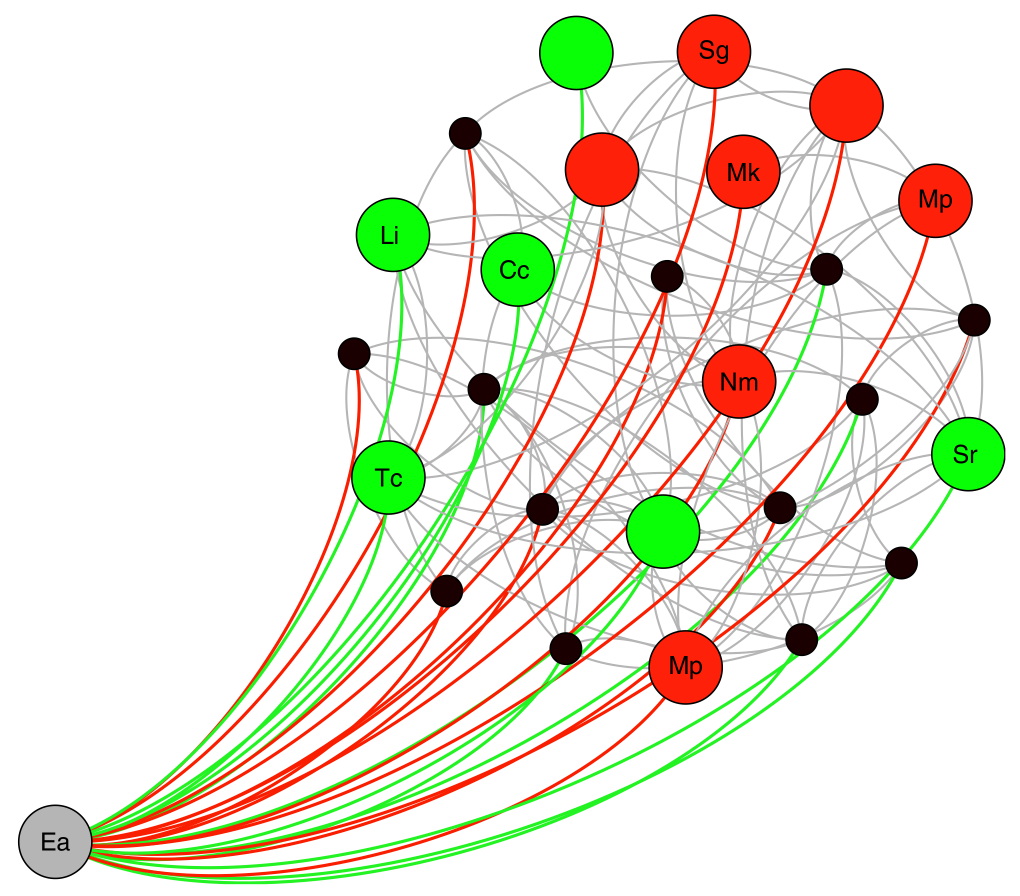
\includegraphics[width=.3\textwidth]{\fignet/JFS16-EnvirMicrobiol-Fig4}
    \end{tabular}
  \end{tabular}

}

  
